\documentclass{article}

\usepackage{graphicx}
\usepackage{mathtools}
\usepackage{hyperref}
\usepackage{amsfonts}
\usepackage{framed}

% Prevent LaTeX from repositioning tables
\usepackage{float}
\restylefloat{table}

% For figures
\usepackage{tikz}
\usetikzlibrary{fit,positioning}
\usetikzlibrary{matrix}
\usetikzlibrary{decorations.pathreplacing}

% Change page size
\usepackage[margin=1.5in]{geometry}

% % % % % % % % % % % % % % % % % % % % % % % % % % % % % % % % % % % % % % % % % %	

\begin{document}
	\title{Latent variable model version of CauseNet}
	\author{Thomas Brouwer, Computer Laboratory}
	\date{}
	\maketitle{}
	
	\section*{Overview}
		The idea is to use penalised non-negative matrix tri-factorisation (PNMTF) on the NCI-60 drug sensitivity dataset. In matrix tri-factorisation we decompose a matrix \( \boldsymbol R_{12} \) relating two entities (1 and 2) into three matrices \( \boldsymbol R_{12} \approx \boldsymbol G_1 \boldsymbol S_{12} \boldsymbol G_2^T \). These matrices capture clusterings of the entities, and then relate those entities, to give the original matrix. By adding extra penalising terms expressing similarity of entities between themselves, we can force similar entities to be clustered together. 
		
		This method was recently used (Gligorijevi\'{c} et al., 2014 \cite{gligorijevic_2014}) for clustering genes and Gene Ontology (GO) terms for genes, and predicting new associations between GO terms.
		
		In this project, we want to apply the PNMTF algorithm to \textbf{predict drug sensitivity values}. We have an incomplete matrix of \( GI_{50} \) drug sensitivity values for a set of drugs and cancer cell lines, as well as a set of drug features and cancer cell line gene expression values. The drug sensitivity matrix is \( \boldsymbol R_{12} \), and we can construct similarity matrices between drugs using the drug features, and similarity matrices between cancer cell lines using the cell line features. Using these similarity matrices we constrain the clustering of drugs and cancer cell lines, and by multiplying the matrices back together we can impute the missing values in \( \boldsymbol R_{12} \). 
		
		In the current literature these methods have either used complete relation matrices, or set the missing values to the row average, which is a great limitation to the algorithm. We will provide an algorithm for PNMTF that can address the issue of missing values.
		
		As far as I am aware, matrix tri-factorisation with missing values has not yet been done.
	
	% % % % % % % % % % % % % % % % % % % % % % % % % % % % % % % % % % % % % % % % % %	
					
	\section{Literature review}
		\subsection{Penalised Non-Negative Matrix Tri-Factorisation}
			The original Non-Negative Matrix Tri-Factorisation (NMTF) algorithm was presented by Ding et al. in 2006 \cite{ding_2006}. Wang et al. demonstrated the use of NMTF for biclustering of data points relating two different entities, and extended the algorithm to include a penalty matrix guiding the clustering of entities that are similar \cite{wang_2008}. This algorithm is called Penalised Non-Negative Matrix Tri-Factorisation (PNMTF). More recently, Gligorijevi\'{c} et al. \cite{gligorijevic_2014} extended PNMTF to allow multiple penalty matrices for the same entity type, and used this method to cluster genes and Gene Ontology (GO) terms.
			
			- A Non-negative Matrix Tri-factorization Approach to Sentiment Classification with Lexical Prior Knowledge
			
			
			
			All of the above papers assume a complete input matrix \( \boldsymbol R_{12} \), and only use the algorithm for biclustering.
	
		\subsection{Drug sensitivity prediction}
	
		What other papers have done drug sensitivity prediction?
		Has (P)NMTF been used for any other problems in Bioinformatics?
		
		\subsection{Drug sensitivity prediction}
		
		\subsection{Performance}
			What performances have been achieved for drug sensitivity prediction? 
			Did these methods give a biological interpretation/insight?
			Can we get the code for these methods?
			What is a good baseline performance?
		
	% % % % % % % % % % % % % % % % % % % % % % % % % % % % % % % % % % % % % % % % % %	
		
	\section{Penalised Non-Negative Matrix Tri-Factorisation}
		\subsection{Non-Negative Matrix Tri-Factorisation}
			Say we have two different types of entities, one consisting of \( n_1 \) unique entities and another consisting of \( n_2 \). We can represent the \textit{inter-type} relationships between these two types of entities as a matrix \( \boldsymbol R_{12} \in \mathbb{R}^{n_1 \times n_2} \), where \( \boldsymbol R_{12}(i,j) \) represents how related entity \( i \) of type 1 is to entity \( j \) of type 2. 
			
			The NMTF algorithm (Ding et al., 2006 \cite{ding_2006}) performs biclustering of the two types of entities -- meaning we cluster in both the rows and the columns of the matrix \( \boldsymbol R_{12}(i,j) \) at the same time. We do this by decomposing the original matrix into three low-rank matrices, such that when we multiply those matrices together we roughly get the original matrix. These matrices cluster the entities together, where the ranks of the matrices determine the number of clusters for each entity type.
			
			\begin{equation*}
				\boldsymbol R_{12} \approx \boldsymbol G_1 \boldsymbol S_{12} \boldsymbol G_2^T
			\end{equation*}
			
			\begin{itemize}
				\item \( \boldsymbol G_1 \in \mathbb{R}_+^{n_1 \times k_1} \) is a non-negative matrix that indicates the clustering of entities of type 1 into \( k_1 \) clusters (soft clustering).
				\item \( \boldsymbol G_2 \in \mathbb{R}_+^{n_2 \times k_2} \) is a non-negative matrix that indicates the clustering of entities of type 2 into \( k_2 \) clusters (soft clustering).
				\item \( \boldsymbol S_{12} \in \mathbb{R}^{k_1 \times k_2} \) is the low-dimensional matrix that represents the original relation matrix \( \boldsymbol R_{12} \), compressed to relate clusters of the two types of entities, rather than entities.
				\item The clustering greatly reduces the dimensions of the data; \( k_1 \ll n_1, k_2 \ll n_2 \).
			\end{itemize}
			
			\begin{figure}[H]
				\centering
				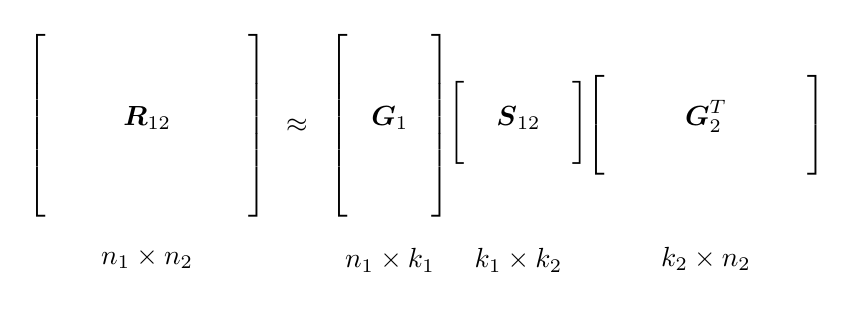
\begin{tikzpicture}
					% R_12
					\matrix (R12) [matrix of nodes, left delimiter  = {[}, right delimiter = {]},
								   text height=10mm, text depth=10mm, text width=20mm, text centered]
					{ \( \boldsymbol R_{12} \) \\ };
					
					\node [right=0.4cm of R12] {\( \approx \)};
					
					% G_1
					\matrix (G1) [right=1.35cm of R12, matrix of nodes, left delimiter  = {[}, right delimiter = {]},
								  text height=10mm, text depth=10mm, text width=5mm, text centered]
					{ \( \boldsymbol G_1 \) \\ };
					
					%\node [right=0.4cm of G1] {\( \times \)};
					
					% S_12
					\matrix (S12) [right=0.5cm of G1, matrix of nodes, left delimiter  = {[}, right delimiter = {]},
								  text height=2.5mm, text depth=2.5mm, text width=8mm, text centered]
					{ \( \boldsymbol S_{12} \) \\ };
										
					%\node [right=0.4cm of S12] {\( \times \)};
					
					% G_2
					\matrix (G2) [right=0.5cm of S12, matrix of nodes, left delimiter  = {[}, right delimiter = {]},
								  text height=4mm, text depth=4mm, text width=20mm, text centered]
					{ \( \boldsymbol G_2^T \) \\ };
					
					% Add dimension labels below matrices
					\node [below=0.2cm of R12] {\( n_1 \times n_2 \)};
					\node [below=0.2cm of G1] {\( n_1 \times k_1 \)};
					\node [below=0.95cm of S12] {\( k_1 \times k_2 \)};
					\node [below=0.78cm of G2] {\( k_2 \times n_2 \)};
				\end{tikzpicture}
			\end{figure}
						
			\noindent \textbf{Note:} This is actually semi-NMTF, because we relaxed the constraint that \( \boldsymbol S_{12} \) has to be nonnegative. \\
			
			\noindent We want to find the matrices \( \boldsymbol G_1, \boldsymbol S_{12}, \boldsymbol G_2^T \) that represent the original relationl matrix \( \boldsymbol R_{12} \) as closely as possible. To do this, we minimise the square error,
			
			\begin{equation}
				\min_{ \boldsymbol G_1 \ge 0, \boldsymbol G_2 \ge 0 } J = { || \boldsymbol R_{12} - \boldsymbol G_1 \boldsymbol S_{12} \boldsymbol G_2^T ||^2 }
			\end{equation}
			
			\noindent This is done by repeatedly performing the following updates.
			
			\begin{equation}
				G_{1ik} \leftarrow G_{1ik} \sqrt{ \displaystyle \frac{ (R_{12} G_2 S_{12}^T)_{ik} }{ (G_1 G_1^T R_{12}^T G_2 S_{12}^T)_{ik} } } 
				\hspace{30pt} ( i=1,..,n_1, k=1,..,k_1 ) 
			\end{equation}
			
			\begin{equation}
				G_{2jk} \leftarrow G_{2jk} \sqrt{ \displaystyle \frac{ (R_{12}^T G_1 S_{12})_{jk} }{ (G_2 G_2^T R_{12}^T G_1 S_{12})_{jk} } } 
				\hspace{30pt} ( j=1,..,n_2, k=1,..,k_2 ) 
			\end{equation}
			
			\begin{equation}
				S_{12kl} \leftarrow S_{12kl} \sqrt{ \displaystyle \frac{ (G_1^T R_{12} G_2)_{kl} }{ (G_1 ^T G_1 R_{12} G_2^T G_2)_{kl} } } 
				\hspace{30pt} ( k=1,..,k_1, l=1,..,k_2 ) 
			\end{equation}
			
			\noindent This algorithm is guaranteed to converge to a local minimum. The matrices \( \boldsymbol G_1, \boldsymbol G_2 \) can be initialised using the Kmeans algorithm. \\
			
			\noindent \textbf{Note:} None of the papers using matrix tri-factorisation take into account missing values in the matrix -- they all assume we are given a complete matrix \( R_{12} \), and only use the method to perform biclustering -- rather than imputing missing values. In section \ref{Dealing with missing values} we will consider how to relax this constraint, and use it for missing value prediction.
			
		\subsection{Adding penalisation}
			Using the simple NMTF algorithm we do not incorporate any prior information about which entities of each type should cluster together, because they are more similar, and which should not, because they are dissimilar. To incorporate this information, we can add penalty matrices \( \boldsymbol \Theta_1, \boldsymbol \Theta_2 \) where the element \( (i,j) \) gives the penalty for clustering together entities \( i \) and \( j \) of type 1 or 2, respectively. If a value is positive, we effectively give a reward for clustering those two entities together. Our minimisation function then becomes:
			
			\begin{equation}
				\min_{ \boldsymbol G_1 \ge 0, \boldsymbol G_2 \ge 0 } J = { || \boldsymbol R_{12} - \boldsymbol G_1 \boldsymbol S_{12} \boldsymbol G_2^T ||^2 } + trace( \boldsymbol G_1^T \boldsymbol \Theta_1 \boldsymbol G_1 ) + trace( \boldsymbol G_2^T \boldsymbol \Theta_2 \boldsymbol G_2 )
			\end{equation}
			
			\noindent It can be shown that the following algorithm will converge to a local minimum.
			
			\begin{framed}
				\noindent \textbf{Inputs: } \( \boldsymbol R_{12}, \boldsymbol \Theta_1, \boldsymbol \Theta_2 \) \\
				\textbf{Outputs: } \( \boldsymbol G_1, S_{12}, G_2 \)
				
				\begin{enumerate}
					\itemsep0em
					\item Initialise \( \boldsymbol G_1, \boldsymbol G_2 \) using Kmeans.
					\item Repeat until convergence:
					\begin{enumerate}
						\itemsep0em
						\item Fix \( \boldsymbol G_1, \boldsymbol G_1 \), update \( \boldsymbol S_{12} \) using:
							\begin{equation*}
								\boldsymbol S_{12} \leftarrow ( \boldsymbol G_1^T \boldsymbol G_1 )^{-1} \boldsymbol G_1^T \boldsymbol R_{12} \boldsymbol G_2 ( \boldsymbol G_2^T \boldsymbol G_2 )^{-1}
							\end{equation*}
						\item Fix \( \boldsymbol G_2, \boldsymbol S_{12} \), update \( \boldsymbol G_1 \) using:
							\begin{equation*}
								\boldsymbol G_{1ik} \leftarrow G_{1ik} \sqrt
									{ \frac{ (R_{12} G_2 S_{12}^T)_{ik}^+ +  [G_1 (S_{12}^T G_2^T G_2 S_{12})^-]_{ik} + (\Theta_1^- G_1)_{ik} }
									{ (R_{12} G_2 S_{12}^T)_{ik}^- +  [G_1 (S_{12}^T G_2^T G_2 S_{12})^+]_{ik} + (\Theta_1^+ G_1)_{ik} } }
							\end{equation*}
							
						\item Fix \( \boldsymbol G_1, \boldsymbol S_{12} \), update \( \boldsymbol G_2 \) using:
							\begin{equation*}
								\boldsymbol G_{2jk} \leftarrow G_{2jk} \sqrt
									{ \frac{ (R_{12}^T G_1 S_{12})_{jk}^+ +  [G_2 (S_{12} G_1^T G_1 S_{12}^T)^-]_{jk} + (\Theta_2^- G_2)_{jk} }
									{ (R_{12}^T G_1 S_{12})_{jk}^- +  [G_2 (S_{12} G_1^T G_1 S_{12}^T)^+]_{jk} + (\Theta_2^+ G_2)_{jk} } }
							\end{equation*}
					\end{enumerate}
				\end{enumerate}
			\end{framed}
			
			\noindent Where the + and - indicate that we split up the original matrix into two matrices consisting of only the positive and negative values respectively, where the negative values are stored as positive values, and all other entries are 0. For a matrix \( \boldsymbol M \), \( \boldsymbol M^+ = \frac{|\boldsymbol M| + \boldsymbol M}{2} \) and \( \boldsymbol M^- = \frac{|\boldsymbol M| - \boldsymbol M}{2} \).
			
			\begin{equation*} 
			\begin{split}
				\boldsymbol \Theta_1 &= \boldsymbol \Theta_1^+ - \boldsymbol \Theta_1^- \\
				\boldsymbol R_{12} \boldsymbol G_2 \boldsymbol S_{12}^T &= (\boldsymbol R_{12} \boldsymbol G_2 \boldsymbol S_{12}^T)^+ - (\boldsymbol R_{12} \boldsymbol G_2 \boldsymbol S_{12}^T)^- \\
				\boldsymbol S_{12}^T \boldsymbol G_2^T \boldsymbol G_2 \boldsymbol S_{12} &= (\boldsymbol S_{12}^T \boldsymbol G_2^T \boldsymbol G_2 \boldsymbol S_{12})^+ - (\boldsymbol S_{12}^T \boldsymbol G_2^T \boldsymbol G_2 \boldsymbol S_{12})^- \\
			\end{split}			
			\end{equation*}
			
		
		\subsection{Multiple penalisation matrices}
			This can be even further extended to allow multiple penalty matrices per entity (Gligorijevi\'{c} et al., 2014 \cite{gligorijevic_2014}). For example, if we have \( m \) constraint matrices \( \{ \boldsymbol \Theta_1^1,..,\boldsymbol \Theta_1^m \} \) for entity 1, our updates for \( G_1 \) become: 
			
			\begin{equation*}
				\boldsymbol G_{1ik} \leftarrow G_{1ik} \sqrt
					{ \frac{ (R_{12} G_2 S_{12}^T)_{ik}^+ +  [G_1 (S_{12}^T G_2^T G_2 S_{12})^-]_{ik} + [(\sum_m \Theta_1^{m-}) G_1]_{ik} }
					{ (R_{12} G_2 S_{12}^T)_{ik}^- +  [G_1 (S_{12}^T G_2^T G_2 S_{12})^+]_{ik} + [(\sum_m \Theta_1^{m+}) G_1]_{ik} } }
			\end{equation*}			
			
			
		\subsection{Dealing with missing values} \label{Dealing with missing values}
			We are ultimately interested in predicting the drug sensitivity values by completing the matrix \( \boldsymbol R_{12} \). However, in order to decompose the matrix we need to know all values. 
			
			Chen et al. (2008 \cite{chen_2007}) dealt with this by setting unknown values to the average of the known values in that row, claiming it performed better than initialising values to zeros, and equally well as the average of the column.
			
			This tactic might work well because we observe rows have largely the same values in the drug sensitivity dataset. However, we will always be limited by this approach -- if our algorithm fit the dataset perfectly, we would get the same performance as simply predicting the average of a row.
			
			
	% % % % % % % % % % % % % % % % % % % % % % % % % % % % % % % % % % % % % % % % % %
			
	\section{PNMTF for Missing Value Prediction}
		Show how to extend NMTF and PNMTF to perform updates with missing values, without having to set those missing values to e.g. 0 or the row/column average.
	
	% % % % % % % % % % % % % % % % % % % % % % % % % % % % % % % % % % % % % % % % % %
					
	\section{Datasets}
		Drug sensitivity values - GI50
		Drug features
		Cancer cell line gene expression values - without the drugs applied to them, raw expression values (not differential, compared to normal cell lines)
	
	% % % % % % % % % % % % % % % % % % % % % % % % % % % % % % % % % % % % % % % % % %		
			
	\section{PNMTF for Drug Sensitivity Prediction}
		Describe how we can use the method for drug sensitivity prediction.
		
		\subsection{Constructing similarity matrices for penalisation}
			How do we use the features to construct (potentially multiple) similarity matrices for penalisation. Construct Laplacian network matrix?
			
		\subsection{Prediction}
			How do we use the three matrices to predict new values. In-matrix prediction should we easy.
			Can we also do out-of-matrix prediction?
			Do we do cross-validation? 
			
			For out-of-matrix prediction, could always train the model using PNMTF to give \( G_1, G_2 \), use Linear Regression with \( Y_1 = G_1, Y_2 = G_2 \) and inputs \( X_1, X_2 \) being the drug features and cell line features resp., to give the weight matrices \( W_1, W_2 \), which we can then use for new drugs and cell lines to give new \( G_1, G_2 \), and multiplying those together gives the predictions for drug sensitivities values.
			
		\subsection{Biological interpretation}
			How can we interpret the clustering matrices \( \boldsymbol G_1 \) and \( \boldsymbol G_2 \)? What biological information does this give us?
	
	% % % % % % % % % % % % % % % % % % % % % % % % % % % % % % % % % % % % % % % % % %
	
	\section{Probabilistic PNMTF}
		NMTF has been put in the probabilistic framework - how about PNMTF?
		See if any papers have done it already.
		If not, think of ways to do it.
		
	% % % % % % % % % % % % % % % % % % % % % % % % % % % % % % % % % % % % % % % % % %
	
	\section{Multi-type PNMTF}
		In Wang et al. (2008 \cite{wang_2008}) a method for PNMTF was given in the case of more than two entity types. Perhaps we could also use this method for drug sensitivity prediction - e.g. clustering drugs with drug targets as well, or genes with pathways. Not entirely convinced this will help though - surely the clustering of one entity i with entity j is independent of the clustering of entity i with entity k, due to the different F and G matrices for all entity type combinations... 
	
	% % % % % % % % % % % % % % % % % % % % % % % % % % % % % % % % % % % % % % % % % %
	
	\section{Project outline}
		\begin{enumerate}
			\item Implement baseline classifier for performance comparison -- e.g. Random Forest on drug and cell line features. Test performance with cross-validation. 
			\item Implement NMTF, using row average and zero for missing values, and run on the drug sensitivity dataset. Compare to baseline performance.
			\item Implement PNMTF, using row average and zero for missing values, construct a constraint matrix for the cell lines, and one for the drugs. Compare performance (should be better than NMTF).
			\item Implement NMTF with missing values, and compare performance to regular NMTF. If better:
			\item Implement PNMTF with missing values.
			\item \textbf{Extension:}  Implement Probabilistic PNMTF, with missing values. 
		\end{enumerate}
	
% % % % % % % % % % % % % % % % % % % % % % % % % % % % % % % % % % % % % % % % % %

\begin{thebibliography}{9}

\bibitem{ding_2006}
  Chris Ding, Tao Li, Wei Peng and Haesun Park.
  \emph{Orthogonal Nonnegative Matrix Tri-factorizations for Clustering}.
  Proceedings of the International Conference on Knowledge Discovery and Data Mining (KDD 2006), ACM Press, New York, 2006, pp. 126–135.
  
\bibitem{chen_2007}
  Gang Chen, Fei Wang, and Changshui Zhang.
  \emph{Collaborative filtering using orthogonal nonnegative matrix tri-factorization}.
  In Proceedings of the IEEE International Conference on Data Mining Workshops, pages 303–308, 2007.
  
\bibitem{wang_2008}
  Fei Wang, Tao Li, and Changshui Zhang.
  \emph{Semi-Supervised Clustering via Matrix Factorization}.
  8th SIAM international conference on data mining.
  
\bibitem{wang_2011}
  Hua Wang, Heng Huang, Chris Ding.
  \emph{Simultaneous Clustering of Multi-Type Relational Data via Symmetric Nonnegative Matrix Tri-Factorization}.
  In ACM International Conference on Information and Knowledge Management (CIKM). 279–284.
  
\bibitem{gligorijevic_2014}
  Vladimir Gligorijevi\'{c}, Vuk Janji\'{c}, and Nata\v{s}a Pr\v{z}ulj.
  \emph{Integration of molecular network data reconstructs Gene Ontology}.
  Bioinformatics, 
  Vol. 30 ECCB 2014, pages i594-i600.
  
  

\end{thebibliography}

\end{document}